\documentclass{article}
\usepackage[utf8]{inputenc}
\usepackage{amsmath}
\usepackage{indentfirst}
\usepackage{graphicx,caption}
\usepackage[a4paper, margin=1in]{geometry}
\linespread{1.15}
\usepackage{empheq}
\usepackage[most]{tcolorbox}
\usepackage[margin=3cm]{caption}
\usepackage{siunitx}
\usepackage{array}
\usepackage{braket}
\usepackage{mathtools}

\usepackage{xcolor,sectsty}
\definecolor{astral}{RGB}{46,116,181}
\subsectionfont{\color{astral}}
\sectionfont{\color{astral}}

\title{
\includegraphics[width=0.1\textwidth]{ufallogo.png} \\
\Huge{\color{astral}\textbf{Métodos Perturbativos em Mecânica Quântica}}}
\author{Paulo Brandão}
\date{Maio de 2017}

\newtcbox{\mymath}[1][]{%
    nobeforeafter, math upper, tcbox raise base,
    enhanced, colframe=blue!30!black,
    colback=blue!30, boxrule=1pt,
    #1}
\newcommand*{\bfrac}[2]{\genfrac{\lbrace}{\rbrace}{0pt}{}{#1}{#2}}
\begin{document}

\maketitle

\section{Introdução}

Com a descoberta das leis e equações diferenciais que regem o comportamento dos átomos e moléculas, o próximo passo para o avanço da teoria é resolver tais equações para determinados sistemas físicos. No domínio da mecânica quântica não-relativística (onde iremos nos concentrar nesta aula), o grande problema é, dadas as condições de contorno para uma única partícula, obter as soluções da equação de Schrödinger para a função de onda $\Psi(\mathbf{r},t)$ tal que a integração do módulo ao quadrado por todo o espaço seja um número finito. Infelizmente, é possível contar nos dedos o número de problemas que podem ser resolvidos dessa maneira de uma forma exata, isto é, sem envolver aproximações. Dessa forma, físicos e matemáticos desenvolveram ferramentas para obter \textit{soluções aproximadas} de equações diferenciais. O objetivo dessa aula é mostrar ao estudante a importância desses métodos de aproximação, ou \textbf{métodos perturbativos}, de um ponto de vista moderno que não é geralmente tratado em livros texto mais conhecidos. Formalmente, a solução de um problema em mecânica quântica por um método perturbativo possui bastantes sutilezas que não são geralmente tratadas num tratamento do ponto de vista físico. Nossa discussão começa na seção 2 com a descrição dos três passos que todo método perturbativo deve possuir. A seção 3 resolve um problema simples utilizando os passos descritos na seção 2 e enfatiza as sutilezas presentes em cada um dos passos. Tais sutilezas estão presentes nos problemas em mecânica quântica e , de fato, em \textbf{todos} os problemas de natureza perturbativa. A discussão do método em teoria quântica começa na seção 4 com a introdução da equação de Schrödinger independente do tempo. A seção 5 aplica os passos descritos na seção 2 para resolver a equação de Schrödinger em sistemas não-degenerados. Calcularemos a perturbação em primeira e segunda ordem na energia e em primeira ordem na função de onda. A aula termina com uma receita na seção 6 para resolver problemas degenerados com uma degenerescência arbitrária entre os estados não-perturbados. 

Após o término desta aula, o estudante estará apto a aplicar métodos de perturbação em problemas gerais descritos por equações diferenciais, equações algébricas ou qualquer outro sistema cuja resposta exata não seja conhecida.

\section{As Três Etapas de um Método Perturbativo}

Vamos supor que estamos interessados em resolver um \textbf{p}roblema \textbf{m}uito \textbf{c}omplicado (PMC) de física-matemática (não necessariamente descrito por uma equação diferencial). Após várias tentativas sem sucesso, decidimos utilizar métodos perturbativos nas equações que dispomos. O grande efeito de um método de aproximação aplicado num problema é \textbf{transformar o PMC em infinitos outros problemas mais simples de se resolver}. Essa transformação de um PMC para infinitos problemas mais simples é alcançada através de três passos:
\begin{enumerate}
    \item Converta o problema original em um problema de perturbação através da introdução de um parâmetro pequeno $\varepsilon$ tal que se conheça a solução do problema para $\varepsilon= 0$.
    \item Assuma uma expressão para a resposta na forma de uma série de perturbação e calcule os coeficientes dessa série.
    \item Obtenha a resposta do problema original através da soma da série de perturbação para o valor apropriado de $\varepsilon$.
\end{enumerate}
Apesar da facilidade de enumerar os três passos, cada um possui várias sutilezas que irão variar dependendo do problema considerado, como iremos verificar mais na frente.




\section{Um Exemplo Simples}

Vamos aplicar os três passos descritos na seção anterior em um problema simples. O objetivo é encontrar a raíz real da equação $x^5 + x = 1$. Esse problema é classificado como um PMC porque não existe uma fórmula que nos forneça as raízes da equação. Fórmulas para as raízes de equações polinomiais só existem para polinômios de até quarta ordem. Por essa razão, classifico este problema como um PMC. Como podemos atacar esse problema utilizando um método perturbativo? 

\subsection{Passo 1}

O primeiro passo descrito na seção anterior é introduzir um parâmetro pequeno $\varepsilon$ tal que a solução do problema para $\varepsilon = 0$ seja conhecida. Existem várias alternativas para esse passo. Eis aqui duas:
\begin{enumerate}
    \item $x^5 + \varepsilon x = 1$,
    \item $\varepsilon x^5 + x = 1$.
\end{enumerate}
No primeiro caso, o parâmetro $\varepsilon$ é colocado multiplicando o termo $x$ e no segundo caso o parâmetro $\varepsilon$ multiplica o termo $x^5$. Como em ambos os casos podemos resolver a equação para $\varepsilon = 0$, o primeiro passo foi concluído com sucesso. Para prosseguir, é mais conveniente escolher uma das duas formas descritas acima. Vamos assumir primeiramente que o parâmetro $\varepsilon$ multiplica o termo $x$. Assim, quando $\varepsilon = 0$ temos que $x^5 = 1$ cuja raíz real vale $x_{0} = 1$. Esse valor representa a solução para o problema \textbf{não-perturbado} ($\varepsilon = 0$) e não é relativamente distante do valor verdadeiro $x_\text{exato} = 0,75487767...$, mas podemos fazer melhor. 

\subsection{Passo 2}

Vamos agora para o segundo passo descrito na seção anterior que diz que devemos assumir uma expansão em série de potências em torno de $\varepsilon = 0$:
\begin{equation}
    x(\varepsilon) = 1 + a\varepsilon + b\varepsilon^2 + c\varepsilon^3 + ...,
    \label{eq1}
\end{equation}
onde o primeiro valor da série é nada mais que o  valor não-perturbado para $\varepsilon = 0$. O próximo objetivo é calcular os coeficientes da série (ainda no Passo 2). Para isso, devemos substituir a série \eqref{eq1} na equação que queremos resolver:
\begin{equation}
    (1 + a\varepsilon + b\varepsilon^2 + c\varepsilon^3 + ...)^5 + \varepsilon(1 + a\varepsilon + b\varepsilon^2 + c\varepsilon^3 + ...)  = 1
\end{equation}
\begin{equation}
    (1-1)\varepsilon^{0} + (5a+1)\varepsilon^{1} + (5b+10a^2 + a)\varepsilon^2 + (5c + 20ab + b + 10a^3)\varepsilon^3 ... = 0
\end{equation}
Precisamos assumir que a expansão em Taylor é única e convergente para igualar os coeficientes à zero. Claro que não sabemos se a série converge porque ainda não sabemos os valores dos coeficientes $a,b,c...$, somente no final poderemos tirar alguma conclusão. Logo,

\begin{center}
\begin{tabular}{ c c c }
 Zero ordem $\varepsilon^0$: & $1 = 1$ & Ok \\ 
 Primeira ordem $\varepsilon^1$: & $5a+1 = 0$ & $a = -\frac{1}{5}$ \\  
 Segunda ordem $\varepsilon^2$: & $5b+10a^2 + a = 0$ & $b = -\frac{1}{25}$ \\
 Terceira ordem $\varepsilon^3$: & $5c + 20ab + b + 10a^3 = 0$ & $c = -\frac{1}{125}$
\end{tabular}
\end{center}
Note como a introdução do método perturbativo decompôs um problema muito complicado em um número infinito de problemas simples. De forma que obtemos a expansão
\begin{equation}
    x(\varepsilon) = 1 - \frac{1}{5}\varepsilon - \frac{1}{25}\varepsilon^2 - \frac{1}{125}\varepsilon^3 + ...
\end{equation}
e o Passo 2 está concluído.

\subsection{Passo 3}

O próximo e último passo é o mais sutil. Note que conseguimos obter uma expressão para a raíz real até a ordem três. O passo 3 diz que devemos somar a série para $\varepsilon = 1$ de modo a obter a raíz para o problema original. Assim, até terceira ordem:
\begin{equation}
    x(1) = 1 - \frac{1}{5} - \frac{1}{25} - \frac{1}{125} = 0,7520
\end{equation}
que é uma boa aproximação para a raíz exata $x_\text{exato} = 0,75487767...$. Poderíamos continuar calculando novos coeficientes na expansão de $x(\varepsilon)$ para obter uma aproximação cada vez melhor.

Vamos supor agora que inserimos o parâmetro $\varepsilon$ multiplicando o termo $x^5$. Neste caso, o aluno irá demonstrar através da resolução da lista de exercícios que a expansão de $x(\varepsilon)$ é dada por
\begin{equation}
    x(\varepsilon) = 1 -\varepsilon + 5\varepsilon^2 - 25\varepsilon^3 + 285\varepsilon^4 + ...
\end{equation}
de forma que
\begin{equation}
    x(1) = 256 \hspace{0.3cm}\text{(????)}
\end{equation}
A diferença entre os dois casos é que, no primeiro, o raio de convergência da série é 1,64938 e, portanto, $\varepsilon = 1$ se encontra dentro do raio, enquanto que no segundo caso, o raio de convergência da série é 0,08192 e, portanto, quando colocamos $\varepsilon = 1$ estamos na verdade fora do raio de convergência. A origem mais profunda dessa divergência no resultado dependendo da posição onde colocamos o parâmetro $\varepsilon$, vem do fato de que, na primeira situação, quando o parâmetro multiplica o termo $x$, o problema não-perturbado ainda contém 5 raízes como solução do problema. Já no segundo caso, onde o parâmetro $\varepsilon$ multiplica o termo $x^5$, o problema não-perturbado ``perde'' quatro raízes quando $\varepsilon = 0$. Em outras palavras, ocorre uma mudança abrupta no comportamento das raízes do problema quando $\varepsilon\rightarrow 0$ e $\varepsilon$ é colocado multiplicando o termo $x^5$. 

O exemplo que acabamos de discutir ilustra de forma geral o que acontece na solução de um problema de forma perturbativa. A escolha da posição do parâmetro $\varepsilon$ pode fornecer uma série convergente ou não dependendo do valor assumido por $\varepsilon$. Entretanto, se nos depararmos, ao final do problema, com uma série divergente, não devemos nos preocupar pois existem técnicas para \textbf{somar séries divergentes}. Essas técnicas não são ensinadas geralmente em cursos formais de mecânica quântica mas são bem conhecidas por matemáticos e físicos-matemáticos que estudam em teoria de campos. As duas técnicas mais conhecidas para somar séries divergentes são as somas de Padé e de Borel. É possível, portanto, aplicar a técnica da soma de Padé na série divergente (6) e obter um resultado significativo próximo do esperado. O estudante que se interessar por tais métodos pode consultar a lista de bibliografias disponibilizada no plano de aula.


\section{A Equação de Schrödinger Independente do Tempo}

O grande objetivo da mecânica quântica não-relativística é: dado um potencial $V(x)$, encontrar a função de onda $\psi(x)$ que satisfaz a equação de Schrödinger independente do tempo
\begin{empheq}[box=\tcbhighmath]{equation}
-\frac{\hbar^2}{2m}\frac{d^2\psi}{dx^2} + V(x)\psi = E\psi,
\label{eq8}
\end{empheq}
onde $E$ é a energia da partícula representada pela função $\psi$, $m$ sua massa e assumimos que a função de onda satisfaz alguma condição de contorno. Com a solução (ou soluções) podemos formar a solução geral dependente do tempo pois as soluções particulares formam uma base. Vamos trabalhar daqui pra frente com apenas uma dimensão espacial $x$ para facilitar a análise. O caso geral pode ser facilmente estendido a partir da análise unidimensional. As condições de contorno que iremos assumir para a Eq. \eqref{eq8} são
\begin{equation}
    \lim_{|x|\rightarrow \infty} \psi(x) = 0,
    \label{eq9}
\end{equation}
ou seja, a função de onda deve ir à zero para $\pm\infty$ de modo que seja de quadrado integrável. Vamos assumir também que $V(x)$ tende à $\infty$ quando $|x|\rightarrow\infty$, ou, em outras palavras, que o potencial é \textit{localizado}.

\begin{figure}[ht]
\centering
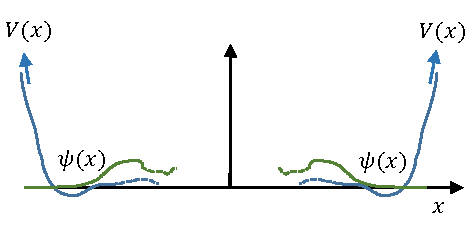
\includegraphics[width=8cm]{fig1.pdf}
\caption{Comportamento do potencial $V(x)$ e da função de onda $\psi(x)$ quando $x\rightarrow\infty$.}
\end{figure}
Com as condições de contorno definidas acima, é possível demonstrar através de uma matemática mais avançada que as soluções da equação de Schrödinger são formadas por funções discretas $\psi_1$, $\psi_2$, $\psi_3$, etc, com energias $E_1$, $E_2$, $E_3$, etc, correspondentes. Iremos assumir que para cada energia exista uma função de onda diferente, isto é, sistema \textit{não é degenerado}. Dessa forma, podemos nomear essas soluções de $\psi_n^{(0)}$ e $E_n^{(0)}$ e reescrever a equação como
\begin{equation}
-\frac{\hbar^2}{2m}\frac{d^2\psi_n^{(0)}}{dx^2} + V(x)\psi_n^{(0)} = H^{(0)}\psi_n^{(0)} =  E_n^{(0)}\psi_n^{(0)},
\end{equation}
Suponha que o potencial $V(x)$ possua uma forma tal que você consiga resolver a Eq. \eqref{eq9} de maneira exata, isto é, que conhecemos explicitamente as funções $\psi_1^{(0)}(x)$, $\psi_2^{(0)}(x)$, etc e $E_1^{(0)}$, $E_2^{(0)}$, etc. Se uma nova força atuar na partícula de interesse, o novo potencial assume uma forma $V(x) + W(x)$ e precisaremos resolver a nova equação de Schrödinger:
\begin{equation}
    \left[ -\frac{d^2}{dx^2} +V(x)+W(x)-E_n \right]\psi_n (x) = 0.
    \label{eq11}
\end{equation}

\section{Método Perturbativo Não-Degenerado}

Note que existem duas quantidades que não conhecemos na Eq. \eqref{eq11}: a função de onda $\psi$ e a energia da partícula $E$. É fácil deduzir que a equação diferencial $\eqref{eq11}$ representa um PMC. Com as condições de contorno adotadas, a teoria matemática diz que existem apenas valores discretos da energia $E_1$, $E_2$, $E_3$, etc, e que, para cada valor de $E$ corresponde uma função de onda $\psi_1$, $\psi_2,$, $\psi_3$ , etc. De que forma podemos resolver esse problema utilizando o método perturbativo? Seguimos os passos descritos anteriormente! O primeiro passo diz que devemos inserir um parâmetro $\varepsilon$ de tal forma que quando $\varepsilon = 0$ conhecemos a solução do problema não-perturbativo. Isso nos força a considerar a única alternativa que é colocar o parâmetro multiplicando a função $W(x)$:
\begin{equation}
    \left[ -\frac{d^2}{dx^2} +V(x)+\varepsilon W(x)-E_n \right]\psi_n (x) = 0.
    \label{eq12}
\end{equation}

Com o primeiro passo concluído, o segundo é escrever uma expansão em série no parâmetro $\varepsilon$. Porém, como temos duas quantidades desconhecidas, $\psi_n$ e $E_n$, expandimos as duas:
\begin{equation}
    \psi_n = \psi_n^{(0)} + \psi_n^{(1)}\varepsilon + \psi_n^{(2)}\varepsilon^2 + ...
    \label{eq13}
\end{equation}
\begin{equation}
    E_n = E_n^{(0)} + E_n^{(1)}\varepsilon + E_n^{(2)}\varepsilon^2 + ...
    \label{eq14}
\end{equation}
A Eq. \eqref{eq12} pode ser reescrita (para facilitar nossos cálculos) na forma
\begin{equation}
    H^{(0)}\psi_n + \varepsilon W \psi_n = E_n \psi_n,
    \label{eq15}
\end{equation}
onde $H^{(0)}$ é o operador Hamiltoniano do sistema não-perturbado, definido acima. Substituindo as Eqs. \eqref{eq13} e \eqref{eq14} na Eq. \eqref{eq15}, obtemos
\begin{multline}
    H^{(0)}(\psi_n^{(0)} + \psi_n^{(1)}\varepsilon + \psi_n^{(2)}\varepsilon^2 + ...) + \varepsilon W (\psi_n^{(0)} + \psi_n^{(1)}\varepsilon + \psi_n^{(2)}\varepsilon^2 + ...) \\
    = (\psi_n^{(0)} + \psi_n^{(1)}\varepsilon + \psi_n^{(2)}\varepsilon^2 + ...)(E_n^{(0)} + E_n^{(1)}\varepsilon + E_n^{(2)}\varepsilon^2 + ...),
\end{multline}
após juntar os termos de mesma ordem e igualar a zero, temos que
\begin{equation}
    \varepsilon^0: \hspace{0.5cm} H^{(0)}\psi_n^{(0)} = E_n^{(0)}\psi_n^{(0)},
\end{equation}
\begin{equation}
    \varepsilon^1: \hspace{0.5cm} H^{(0)}\psi_n^{(1)} + W\psi_n^{(0)} = E_n^{(0)}\psi_n^{(1)} + E_n^{(1)}\psi_n^{(0)},
    \label{eq18}
\end{equation}
\begin{equation}
    \varepsilon^2: \hspace{0.5cm} H^{(0)}\psi_n^{(2)} + W\psi_n^{(1)} = E_n^{(0)}\psi_n^{(2)} + E_n^{(1)}\psi_n^{(1)} + E_n^{(2)}\psi_n^{(2)}.
\end{equation}
Claramente o problema fica mais complicado a medida que calculamos termos de ordens mais altas. Na ordem zero não obtemos nenhuma novidade, apenas a equação de Schrödinger não-perturbada, cujas soluções $\psi_n^{(0)}$ já conhecemos. 

\subsection{Perturbação de Primeira Ordem}

Se considerarmos o termo de primeira ordem \eqref{eq18}, é fácil perceber que existem duas variáveis desconhecidas na equação: $\psi_n^{(1)}$ e $E_n^{(1)}$. O truque para escrever a energia de primeira ordem $E_n^{(1)}$ em termos de quantidades conhecidas é multiplicar a Eq. \eqref{eq18} por $(\psi_n^{(0)})^{*}$ e integrar em $x$. O primeiro termo do lado esquerdo fica:
\begin{equation}
    \int_{-\infty}^{+\infty}(\psi_n^{(0)})^{*}H^{(0)}\psi_n^{(1)}dx = \braket{\psi_n^{(0)}|H^0|\psi_n^{(1)}} = E_n^{(0)}\braket{\psi_n^{(0)}|\psi_n^{(1)}}.
\end{equation}
O segundo termo:
\begin{equation}
    \int_{-\infty}^{+\infty}(\psi_n^{(0)})^{*}W\psi_n^{(0)}dx = \braket{\psi_n^{(0)}|W|\psi_n^{(0)}}.
\end{equation}
O terceiro termo
\begin{equation}
    \int_{-\infty}^{+\infty}(\psi_n^{(0)})^{*}E_n^{(0)}\psi_n^{(1)}dx = E_n^{(0)}\braket{\psi_n^{(0)}|\psi_n^{(1)}}
\end{equation}
cancela o primeiro termo do lado esquerdo. O quarto termo é trivial e vale $E_n^{(1)}$, de modo que obtemos a primeira correção para a energia: $E_n^{(1)} = \braket{\psi_n^{(0)}|W|\psi_n^{(0)}}$, ou
\begin{equation}
\begin{split}
    E_n(\varepsilon) &= E_n^{(0)} + \varepsilon\braket{\psi_n^{(0)}|W|\psi_n^{(0)}} + \varepsilon^2 (??) + ... \\
                     &= E_n^{(0)} + \varepsilon\int_{-\infty}^{+\infty}(\psi_n^{(0)})^{*}W\psi_n^{(0)}dx + \varepsilon^2 (??) + ...
\end{split}
\end{equation}

Para obter a primeira correção $\psi_n^{(1)}$ para a função de onda, o truque é reescrever a Eq. \eqref{eq18} na forma
\begin{equation}
    (H^{(0)} - E_n^{(0)})\psi_n^{(1)} =- (W - E_n^{(1)}) \psi_n^{(0)}.
    \label{eq24}
\end{equation}
O lado direito é conhecido e a equação acima representa uma equação diferencial não-homogênea para $\psi_n^{(1)}$, a função que queremos encontrar. O truque para resolver esse problema é lembrar que as funções de onda do problema não-perturbar, $\psi_n^{(0)}$, formam uma base e podemos portanto escrever a função $\psi_n^{(1)}$ como combinação linear delas:
\begin{equation}
    \psi_n^{(1)} = \sum_m c_m^n \psi_m^{(0)} = c_n^n \psi_n^{(0)} + \sum_{m\neq n} c_m^n \psi_m^{(0)},
    \label{eq25}
\end{equation}
onde retirei o termo $m = n$ da soma pois ele não irá contribuir para a solução final, como ficará mais claro adiante. Substituindo a Eq. \eqref{eq25} na Eq. \eqref{eq24},
\begin{equation}
    (H^{(0)} - E_n^{(0)})\left( c_n^n \psi_n^{(0)} + \sum_{m\neq n} c_m^n \psi_m^{(0)} \right) = - (W - E_n^{(1)}) \psi_n^{(0)}
\end{equation}
\begin{equation}
    (H^{(0)} - E_n^{(0)})c_n^n \psi_n^{(0)} + (H^{(0)} - E_n^{(0)})\sum_{m\neq n} c_m^n \psi_m^{(0)}  = - (W - E_n^{(1)}) \psi_n^{(0)}.
\end{equation}
O primeiro termo do lado esquerdo é nulo e isso justifica a remoção do termo $m=n$ do somatório descrito na Eq. \eqref{eq25}. Ficamos com
\begin{equation}
    (H^{(0)} - E_n^{(0)})\sum_{m\neq n} c_m^n \psi_m^{(0)}  = - (W - E_n^{(1)}) \psi_n^{(0)},
\end{equation}
\begin{equation}
    \sum_{m\neq n} (E_m^{(0)} - E_n^{(0)}) c_m^n \psi_m^{(0)}  = - (W - E_n^{(1)}) \psi_n^{(0)}.
    \label{eq29}
\end{equation}
Agora multiplicamos a Eq. \eqref{eq29} por $(\psi_l^{(0)})^{*}$ e integramos em $x$ para obter
\begin{equation}
    \sum_{m\neq n} (E_m^{(0)} - E_n^{(0)}) c_m^n \braket{\psi_l^{(0)}|\psi_m^{(0)}}  = -\braket{\psi_l^{(0)}|W|\psi_n^{(0)}} + \braket{\psi_l^{(0)}|\psi_n^{(1)}}E_n^{(1)}.
\label{eq30}
\end{equation}
Se $l = n$, o lado esquerdo da Eq. \eqref{eq30} é nulo (verifique), de forma que obtemos a correção para a energia de primeira ordem que já conhecemos. Se $l\neq n$, então
\begin{equation}
    (E_l^{(0)} - E_n^{(0)}) c_l^n = -\braket{\psi_l^{(0)}|W|\psi_n^{(0)}},
\end{equation}
como o índice $l$ é mudo, podemos chamá-lo de $m$ novamente, de forma que
\begin{equation}
    (E_m^{(0)} - E_n^{(0)}) c_m^n = -\braket{\psi_m^{(0)}|W|\psi_n^{(0)}}.
\end{equation}
Como estamos assumindo que cada estado $\psi_n^{(0)}$ da solução não-perturbada tem como correspondente uma energia $E_n^{(0)}$ única (não há degenerescência, isto é, dois estados diferentes sempre possuirão duas energias diferentes), podemos dividir a expressão acima por $E_m^{(0)} - E_n^{(0)}$ para obter
\begin{equation}
    c_m^n = \frac{\braket{\psi_m^{(0)}|W|\psi_n^{(0)}}}{(E_n^{(0)} - E_m^{(0)})}.
\end{equation}
A correção em primeira ordem da função de onda $\psi_n$ pode ser escrita como 
\begin{equation}
    \psi_n^{(1)} = \sum_{m\neq n} \frac{\braket{\psi_m^{(0)}|W|\psi_n^{(0)}}}{(E_n^{(0)} - E_m^{(0)})} \psi_m^{(0)},
\end{equation}
ou
\begin{equation}
    \psi_n(x;\varepsilon) = \psi_n^{0}(x) + \varepsilon\sum_{m\neq n} \frac{\braket{\psi_m^{(0)}|W|\psi_n^{(0)}}}{(E_n^{(0)} - E_m^{(0)})} \psi_m^{(0)} + \varepsilon^2 (??) + ...
\end{equation}
Em resumo, com a teoria de perturbação de primeira ordem podemos calcular
\begin{empheq}[box=\tcbhighmath]{equation}
E_n (\varepsilon) = E_n^{(0)} + \varepsilon\braket{\psi_n^{(0)}|W|\psi_n^{(0)}} + \varepsilon^2 (??) + ...
\end{empheq}
\begin{empheq}[box=\tcbhighmath]{equation}
    \psi_n(x;\varepsilon) = \psi_n^{0}(x) + \varepsilon\sum_{m\neq n} \frac{\braket{\psi_m^{(0)}|W|\psi_n^{(0)}}}{(E_n^{(0)} - E_m^{(0)})} \psi_m^{(0)} + \varepsilon^2 (??) + ...
\end{empheq}

\subsection{Perturbação de Segunda Ordem}

Os passos para o cálculo da correção da energia e da função de onda em segunda ordem serão feitos pelo estudante através da resolução da lista de exercícios. A derivação das correções não envolve nenhum princípio novo e com o material desenvolvido até esse ponto é possível derivar as novas correções. Assim, apenas mostrarei o resultado para a correção de segunda ordem da energia:
\begin{empheq}[box=\tcbhighmath]{equation}
E_n (\varepsilon) = E_n^{(0)} + \varepsilon\braket{\psi_n^{(0)}|W|\psi_n^{(0)}} + \varepsilon^2 \sum_{m\neq n} \frac{|\braket{\psi_m^{(0)}|W|\psi_n^{(0)}}|^{2}}{E_n^{(0)} - E_m^{(0)}} + \varepsilon^3 (??) + ...
\end{empheq}


\section{Método Perturbativo Degenerado}

Assumimos na discussão anterior que todas as funções de onda $\psi_{n}^{(0)}$ do problema não-perturbado correspondiam à valores diferentes das energias $E_n^{(0)}$, isto é, o sistema não possuia degenerescência. Um exemplo de sistema não-degenerado é a partícula dentro de uma caixa unidimensional no intervalo $0<x<a$. As funções de onda e as energias para esse problema são 
\begin{equation}
    \psi_n(x) = \sqrt{\frac{2}{a}}\sin\left( \frac{n\pi }{a}x \right)
\end{equation}
e
\begin{equation}
    E_n^{(0)} = \frac{n^2 \pi^2 \hbar^2}{2ma^2}.
\end{equation}
Como $n$ é um inteiro positivo, cada número distinto de $n$ corresponde a funções e energias distintas, ou seja, o sistema não possui degenerescência. Essa propriedade está ilustrada na Figura 2. Por outro lado, se a partícula estiver confinada em uma caixa em três dimensões, surge uma degenerescência no estado excitado. Neste caso, são necessários três números inteiros positivos ($n_x$,$n_y$,$n_z$) para caracterizar o sistema. A função de onda estacionária e a energia da partícula são dadas por
\begin{equation}
    \psi_{n_x n_y n_z}^{(0)}(x,y,z) = \left(\frac{2}{a}\right)^{3/2} \sin\left( \frac{n_x\pi x}{a} \right) \sin\left( \frac{n_y\pi y}{a} \right) \sin\left( \frac{n_z\pi z}{a} \right)
\end{equation}
e
\begin{equation}
    E_{n_x n_y n_z}^{(0)} = \frac{\pi^2 \hbar^2}{2ma^2}(n_x^2 + n_y^2 + n_z^2).
\end{equation}
O estado fundamental da partícula numa caixa em três dimensões $(n_x,n_y,n_z)=(1,1,1)$ não é degenerado, porém o primeiro estado excitado tem degenerescência tripla: $\psi_{211}^{(0)}$, $\psi_{121}^{(0)}$ e $\psi_{112}^{(0)}$ são estados diferentes com a mesma energia $E = E_{211}^{(0)} = E_{121}^{(0)} = E_{112}^{(0)} = 3\pi^2\hbar^2/ma^2$. Após perturbar o sistema, não podemos aplicar o método descrito nas seções anteriores porque alguns termos do somatório divergem. O objetivo dessa última parte da aula é mostrar como calcular as correções de energias de estados degenerados.

\begin{figure}[ht]
\centering
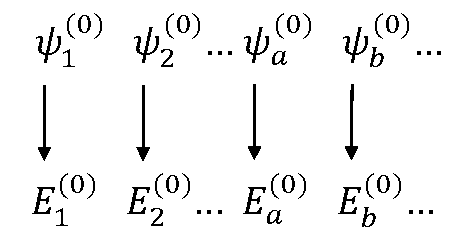
\includegraphics[width=5cm]{fig2.pdf}
\caption{A linha de cima mostra as funções de onda soluções do problema não-perturbado. Para cada função de onda corresponde uma energia diferente, mostradas na linha de baixo. O sistema não é degenerado.}
\end{figure}

Vamos assumir que o sistema não-perturbado possui dois estados $\psi_a^{(0)}$ e $\psi_b^{(0)}$ com a mesma energia $E^{(0)}$, como indica a Figura 3 (degenerescência dupla). Observe inicialmente que se $H^{(0)}\psi_a^{(0)} = E^{(0)}\psi_a^{(0)}$ e $H^{(0)}\psi_b^{(0)} = E^{(0)}\psi_b^{(0)}$, então \textbf{qualquer outro estado escrito na forma}
\begin{equation}
    \psi_{\alpha\beta}^{(0)} = \alpha\psi_a^{(0)} + \beta\psi_b^{(0)}
\end{equation}
\textbf{também possui energia} $E^{0}$ (verifique!). Assim, antes de introduzirmos uma perturbação no problema, não sabemos quais desses infinitos estados o sistema está. O efeito da introdução de um parâmetro $\varepsilon$ é quebrar essa degenerescência na energia $E^{(0)}$, como ilustra a Figura 4. Como não sabemos exatamente o estado inicial com $\varepsilon = 0$, um dos objetivos é encontrar os valores de $\alpha$ e $\beta$ junto com a correção de primeira ordem da energia $E^{(1)}$. 

\begin{figure}[h]
\centering
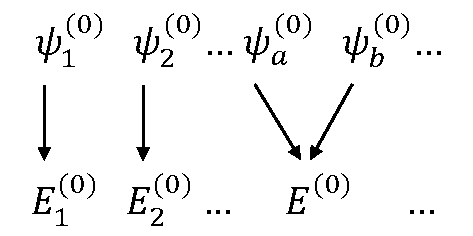
\includegraphics[width=5cm]{fig3.pdf}
\caption{A linha de cima mostra as funções de onda soluções do problema não-perturbado. As funções de onda $\psi_a^{(0)}$ e $\psi_b^{(0)}$ possuem a mesma energia $E^{(0)}$. O sistema é degenerado.}
\end{figure}

Para isso, fazemos novamente a expansão \footnote{Note que agora só estamos considerando os estados degenerados e a energia degenerada. Todos os outros estados e energias que não são degenerados podem ser tratados pela teoria da perturbação descrita nas seções anteriores.}
\begin{equation}
    \psi = (\alpha\psi_a^{(0)} + \beta\psi_b^{(0)}) + \varepsilon\psi^{(1)} + \varepsilon^{2}\psi^{(2)} + ...
\end{equation}
\begin{equation}
    E = E^{(0)} + \varepsilon E^{(1)} + \varepsilon^{2} E^{(2)} + ...
\end{equation}
Substituindo as expansões na equação perturbada, $(H^{(0)} + \varepsilon W)\psi = E\psi$, e, após coletar os termos de primeira ordem em $\varepsilon$ ficamos com (ver lista de exercícios)
\begin{equation}
    H^{(0)}\psi^{(1)} + \alpha W\psi_a^{(0)} + \beta W\psi_b^{(0)} = E^{(0)}\psi^{(1)} + E^{(1)}\alpha\psi_a^{(0)} + E^{(1)}\beta\psi_b^{(0)}.
\end{equation}
Se tomarmos o produto interno da equação acima com $\psi_a^{(0)}$, ficamos com
\begin{equation}
    \alpha W_{aa} + \beta W_{ab} = \alpha E^{(1)},
\end{equation}
e com $\psi_b^{(0)}$ obtemos
\begin{equation}
    \alpha W_{ba} + \beta W_{bb} = \beta E^{(1)},    
\end{equation}
onde $W_{ij} = \braket{\psi_i^{(0)}|W|\psi_j^{(0)}}$ \textit{são conhecidos}. Podemos escrever as duas equações acima em forma matricial:
\begin{equation}
    \begin{bmatrix}
    W_{aa} & W_{ab} \\
    W_{ba} & W_{bb}
\end{bmatrix}
    \begin{bmatrix}
    \alpha  \\
    \beta 
\end{bmatrix} 
=
E^{(1)}    \begin{bmatrix}
    \alpha  \\
    \beta 
\end{bmatrix} .
\end{equation}
Consequentemente, os dois autovalores da matriz $W_{ij}$ representam as correções de energia em primeira ordem do sistema. Eles são dados por:
\begin{equation}
    E^{(1)}_\pm = \frac{1}{2}\left[ W_{aa} + W_{bb} \pm \sqrt{(W_{aa}-W_{bb})^{2} + 4|W_{ab}|^2} \right].
\end{equation}
A correção para a energia, em primeira ordem, vale então
\begin{equation}
    E(\varepsilon) = E^{0} + \varepsilon\bfrac{E^{1}_{+}}{E^{1}_{-}} + ...
\end{equation}

\begin{figure}[ht]
\centering
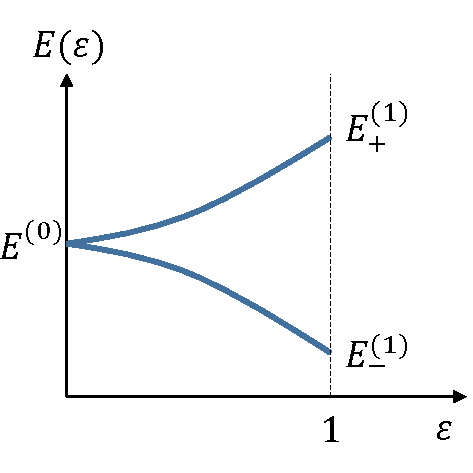
\includegraphics[width=5cm]{fig4.pdf}
\caption{Quebra de degenerescência com o aumento do parâmetro perturbativo $\varepsilon$ para a energia inicialmente degenerada $E^{(0)}$.}
\end{figure}

Para se obter os valores de $\alpha$ e $\beta$ basta calcular os autovetores da matriz $W_{ij}$ para os respectivos valores de energia. O tratamento pode ser estendido para qualquer tipo de degenerescência. Por exemplo, se três estados forem degenerados, $\psi_{a}^{(0)}$, $\psi_{b}^{(0)}$ e $\psi_{c}^{(0)}$ com energia $E^{(0)}$ então é necessário calcular a matriz $3\times 3$
\begin{equation}
    \begin{bmatrix}
    W_{aa} & W_{ab} & W_{ac} \\
    W_{ba} & W_{bb} & W_{bc} \\
    W_{ca} & W_{cb} & W_{cc}
    \end{bmatrix}
\end{equation}
cujos autovalores serão as correções de primeira ordem e os autovetores os coeficientes $\alpha,\beta,\gamma$ da expansão do estado inicial não-degenerado $\psi^{0} = \alpha \psi_{a}^{(0)} + \beta \psi_{b}^{(0)} + \gamma\psi_{a}^{(0)}$.

\section{Conclusões}

O método perturbativo de solução de equações (algébricas ou diferenciais) é muito poderoso porque são raros os casos onde conseguimos resolver equações mais complicadas de forma exata. Todo método perturbativo segue os três passos descritos na segunda seção. Uma aplicação ainda mais interessante ocorre quando consideramos a equação de Schrödinger \textbf{dependente do tempo}. Por conta do tempo de aula não conseguimos discutir esse caso muito importante. Caso o estudante queira se aprofundar nesses conceitos, deve consultar as referências apresentadas no plano de aula.














\end{document}
